\documentclass[a4paper,12pt]{article}
\usepackage{style}
\usepackage{cite}

\begin{document}
    \docNumber{RU.17701729.04.03-01 81 01-1}
    \docFormat{Пояснительная записка}
    \student{БПИ 199}{Д.А. Щербаков}
    \project{Модуль для мобильных приложений для определения эмоционального отклика по изображению пользователя.}
    \supervisor{Аналитик-разработчик \par АО <<Тинькофф банк>>}
    {Весельев А.Н.}
%    \firstPage
%    \newpage
    \annotation
    \section*{Аннотация}
    Данный документ содержит пояснительную записку к модулю <<Facial Expression Recognition Mobile Library>> (<<Модуль для мобильных приложений для определения эмоционального отклика по изображению пользователя>>).
    Модуль служит для определения эмоций человека по изображению его лица, в том числе в режиме реального времени (например, по изображению с камеры).
    В разделе <<Введение>> текущего документа указано наименование программы и документы, на основании которых ведется разработка.
    Раздел <<Назначение и область применения>> содержит функциональное и эксплуатационное назначение ПО и краткую характеристику области применения.
    Раздел <<Технические характеристикии>> описывает постановку задачи на разработку, описание алгоритмов и схему функционирования программы, методы организации входных и выходных данных, состав технических и программных средств и обоснование выбора алгоритма, метода организации ввода и вывода и состава технических средств.
    В разделе <<Технико-экономические показатели>> отражены предполагаемая потребность и экономические преимущества разработки в сравнении с аналогами.
    Настоящий документ разработан в соответствии с требованиями:
    \begin{enumerate}
        \item ГОСТ 19.101-77 Виды программ и программных документов~\cite{gost1};
        \item ГОСТ 19.103-77 Обозначения программ и программных документов~\cite{gost2};
        \item ГОСТ 19.102-77 Стадии разработки~\cite{gost3};
        \item ГОСТ 19.104-78 Основные надписи~\cite{gost4};
        \item ГОСТ 19.105-78 Общие требования к программным документам~\cite{gost5};
        \item ГОСТ 19.106-78 Требования к программным документам, выполненным печатным способом~\cite{gost6};
        \item ГОСТ 19.404-79 Пояснительная записка. Требования к содержанию и оформлению~\cite{gost7};
    \end{enumerate}
    \newpage
%    \thirdPage
%    \newpage

    \section{Введение}

    \subsection{Наименование программы}
    Наименование программы: <<Модуль для мобильных приложений для определения эмоционального отклика по изображению пользователя>>.
    Краткое наименование --\\
    <<facialExpressionRecognitionLib>>.

    \subsection{Документы, на основании которых ведется разработка}
    Основанием для разработки является учебный план подготовки бакалавров по направлению 09.03.04 <<Программная инженерия>> и утвержденная академическим руководителем тема курсового проекта <<Модуль для мобильных приложений для определения эмоционального отклика по изображению пользователя>>.
    \newpage

    \section{Назначение и область применения}

    \subsection{Назначение программы }

    \subsubsection{Функциональное назначение}
    Модуль позволяет определить эмоции человека на изображении по заданной шкале эмоций.

    Прилагаемый к модулю пример эксплуатации позволяет определять эмоциональный отклик на различные записи в социальной сети <<Reddit>> с помощью данных с камеры пользователя.

    \subsubsection{Эксплуатационное назначение}
    Модуль и пример использования должны эксплуатироваться на смартфонах под управлением операционной системы Android.

    \subsubsection{Область применения}
    Программа может быть использована в мобильных приложениях для Android в качестве аналитического модуля для улучшения пользовательского опыта или сбора информации о предпочтениях пользователя.

    \newpage

    \section{Технические характеристики}

    \subsection{Постановка задачи на разработку программы и программного модуля}
    Разработать программный модуль для использования в программах для смартфонов под управлением операционной системы Android с целью анализа эмоций пользователя по его изображению.

    Разработать пример эксплуатации модуля в виде программы для смартфона под управлением операционной системы Android, который позволяет определять эмоциональный отклик на различные записи в социальной сети <<Reddit>> с помощью данных с камеры пользователя.

    \subsection{Описание алгоритмов и функционирования программного модуля}

    \subsubsection{Описание алгоритмов программного модуля}

    \paragraph{Описание алгоритма работы алгоритма для распознавания эмоций на изображении лица}
    \ \vspace{.5em}

    Для распознавания эмоций по изображению используются сверточные нейронные сети (Convolutional Neural Networks).

    Так как создание архитектуры нейронной сети -- трудоемкая задача, в основу данного программного модуля легла архитектура, предложенная исследователями Octavio Arriaga, Matias Valdenegro-Toro и Paul Plöger~\cite{arch}.
    Она, в свою очередь, опирается на еще более фундаментальные труды в области нейронных сетей и машинного обучения, такие как Xception~\cite{xception} и Mobilenets~\cite{mobilenets}.

    Отличительной особенностью данной архитектуры является ее простота в сравнении со state-of-the-art архитектурами (то есть самыми точными) при довольно высокой точности.
    Такой результат достигается за счет более эффективной утилизации признаков -- например, использование разделенных по глубине сверток или отсутствие полносвязных слоев.

    Ниже кратко описаны подходы, используемые в данной нейросети для распознавания эмоций по изображению лица человека.

    \textbf{Разделенные по глубине свертки} -- метод, при котором для входного сигнала используются две матрицы свертки.
    Одна поточечно для каждой карты признаков, а другая -- в глубину между полученными результатами.
    Такой подход позволяет сократить количество операций при большем количестве признаков.
    В приведенной модели данная свертка используется множество раз на тензорах с глубиной 64--128, так что использование разделенной свертки значительно ускоряет время работы сети.

    \textbf{Глобальный пулинг средних} (Global average pooling) -- операция, обычно используемая для классификации вместо полносвязных слоев.
    Обычно в последних слоях нейросети используют полносвязные слои, на вход нейронов которых подаются все извлеченные признаки с предыдущего слоя.
    Такие слои требуют множества вычислений, поэтому для упрощения было предложено использовать метод глобального пулинга - когда последний слой содержит столько карт признаков, сколько мы имеем классов, и затем из каждой карты извлекается среднее и передается в функцию активации.

    \textbf{Остаточные блоки} (Residual blocks) -- блоки нейросети, используемые для того, чтобы нейросеть при увеличении слоев не теряла точности.
    В таких блоках результат получается сложением с функцией идентичности $F(x) = H(x) + x$.
    В современном распознавании изображений с помощью нейронных сетей сложно обойтись без таких блоков \cite{resnet}.

    \begin{figure}[h]
        \caption{Схема приведенной нейронной сети}
        \centering
        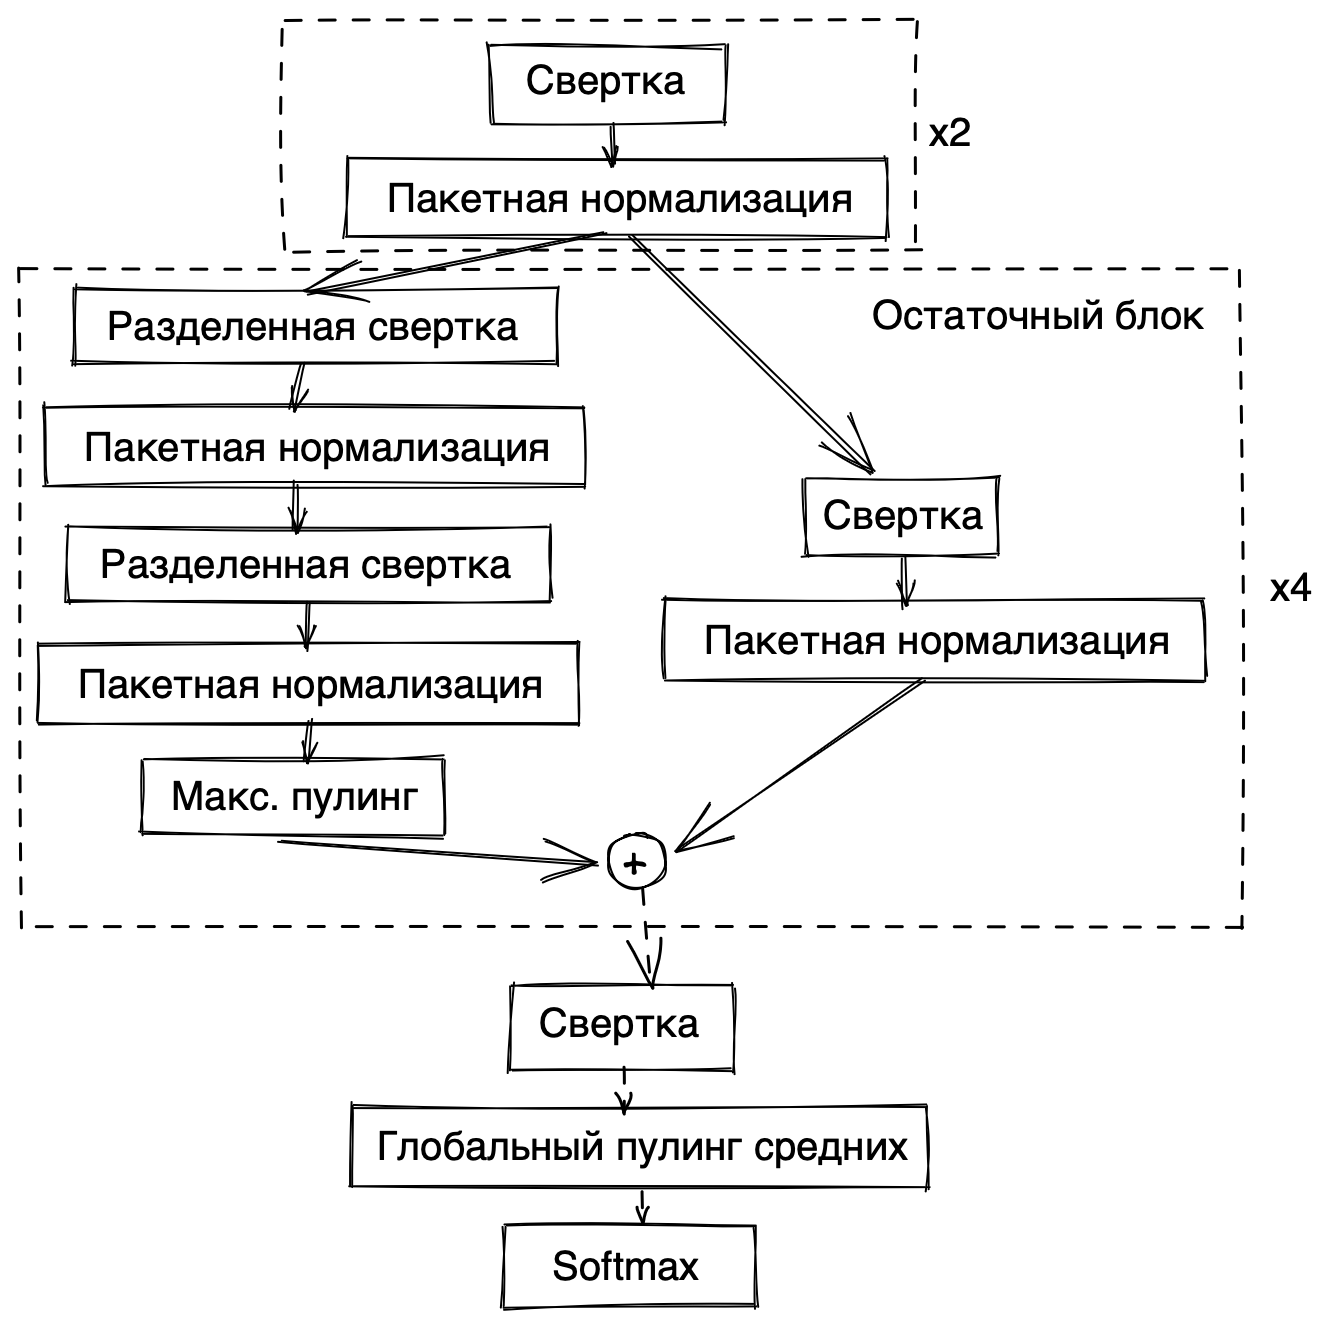
\includegraphics[width=0.75\textwidth]{cnn}
    \end{figure}

    На вход нейросети подается изображение в виде тензора формата float размера 1x1x44x44, соответствующие черно-белой картинке размера 44x44.
    На выходе мы получаем тензор размера 1x1x1x7 и извлекаем из него комбинации из 7 различных эмоций.

    Для обучения сети используется метод оптимизации <<стохастический градиентный спуск>> и функция для минимизации <<перекрестная энтропия>>.
    Это довольно стандартные методы для машинного обучения классификаторов с заданным количеством классов.

    \subsubsection{Обоснование выбора алгоритмов программного модуля}

    \paragraph{Обоснование выбора алгоритма для распознавания эмоций на изображении лица}
    \ \vspace{.5em}

    Сверточные нейронные сети являются очень эффективным инструментом для распознования различных характеристик на изображениях.

    Выбор в пользу конкретной архитектуры был сделан из-за ее высокого соотношения точности на программную сложность.
    Малое количество слоев и параметров и отсутствие полносвязных слоев слоев позволяет быстрее реализовать и обучить нейросеть,
    а также ускоряет ее работу и уменьшает требуемый для работы размер оперативной памяти устройства.

    Скорость работы и объем используемой памяти очень критичны для мобильных устройств, имеющих слабые процессоры и работающих от аккумуляторной батареи.
    На устройстве Huawei Honor 10 с процессором Kirin 970 и при использовании аппаратного ускорения нейронных сетей (технология NNAPI) нейросеть обрабатывает
    изображение размером 44x44 пикселя за менее чем 50 мс, что является удовлетворительным результатом для работы в режиме реального времени.

    \subsubsection{Описание схемы функционирования программного модуля}

    Обученная модель комплируется в JIT-оптимизированный формат вычислительных программ TorchScript~\cite{torchscript}, который можно запустить с помощью библиотеки pytorch\_ android.
    На устройстве под управлением Android такие скрипты выполняются на CPU и по возможности используют модуль нейронных сетей с помощью NNAPI~\cite{nnapi}.

    Для выделения лица на фото используется библиотека MLKit, которая также работает с помощью нейросетей.
    Данная библиотека предоставляет высокоуровневое API для анализа изображений в асинхронном режиме и различными методами распознавания объектов,
    и в рамках данного проекта углубляться в архитектуру этой библиотеки не выглядит целесообразным.

    После выделения прямоугольника, в котором находится лицо, необходимо извлечь эту часть изображения и преобразовать ее в тензор, который будет использоваться моделью.
    Изображения с камеры на смартфонах под управлением Android поступают в формате YUV\_420\_888, что означает, что каждое изображение состоит из трех буферов, которые с помощью специальных алгоритмов объединяются для вывода на экран.
    В случае приведенной модели используется черно-белое изображение, поэтому достаточно извлечь только информацию из первого буфера, или Y-буфера, в котором содержится яркость каждого отдельного пикселя, и перевести это число в формат float, нормализовав по модулю 255.
    Выбираются только те пиксели, что содержат лицо, и ужимаются в небольшой квадрат размером 44x44 пикселя с помощью операций сжатия и растяжения.
    Далее с помощью библиотеки Pytorch тензор передается в модель, и на выходе получается вектор длины 7, в каждой ячейке которого содержится вес определенной эмоции.
    Впоследствии этот вектор можно интерпретировать по-разному, например, выбрать самое большое число в качестве главной эмоции, или выбрать только те значения, что выше какого-либо порога.
    В приведенном примере программы выбирается наибольшее число и конвертируется в строку -- например, первому значению соответствует эмоция ''Злость''.

    \subsection{Описание и обоснование выбора метода организации входных и выходных данных}

    \subsubsection{Описание метода организации входных и выходных данных}

    В модуль на вход может подаваться изображение в формате YUV\_420\_888.
    Также в модуле имеются средства для инициализации камеры и непосредственного анализа информации с нее.

    В качестве выходных данных модуль передает вектор длины 7 с числами от 0 до 1, каждое из которых соответствует вероятности распознанной эмоции из набора стандартных эмоций.

    \subsubsection{Обоснование выбора метода организации входных и выходных данных}

    Формат YUV\_420\_888 является основым стандартом изображений с камеры для смартфонов на ОС Android.

    Полученный с помощью Softmax вектор с весами различных классов -- стандартная практика при решении задач классификации.

    \subsection{Описание и обоснование выбора состава технических и программных средств}

    \subsubsection{Состав технических и программных средств}
    Для работы программного модуля необходим следующий набор программных средств:
    \begin{enumerate}
        \item операционная система Android версии 8.0 и выше
    \end{enumerate}

    Для работы программного модуля необходим следующий состав технических средств:
    \begin{enumerate}
        \item Не менее 512МБ ОЗУ;
        \item Не менее 150МБ свободного места на внутреннем накопителе;
    \end{enumerate}

    Минимальное количество памяти ОЗУ, необходимое для работы системы Android 8.0 и выше составляет 512МБ~\cite{AndroidReq}.

    \newpage
    \section{Технико-экономические показатели}

    \subsection{Предполагаемая потребность}
    Данный программный модуль позволит разработчикам приложений для Android быстро и легко решить задачу распознавания эмоций пользователя.

    \subsection{Экономические преимущества разработки и аналоги}
    Преимущества данного модуля заключаются в быстродействии анализатора, а также в легкой интеграции с программами для ОС Android.
    Других общедоступных библиотек, включающих в себя все функции данного модуля, такие как: предварительная обработка изображения, подключение к камере и запуск модели, найдено не было.
    Экономическая выгода использования данной разработки заключаются в экономии времени разработчиков приложений.
    \\

    \noindent
    \begin{tabular}{| l | c | c | c | c | c |}
        \hline
        & \parbox[c][2cm][c]{2.2cm}{\centering Подготовка изображения}
        & \parbox[c][2cm][c]{2.2cm}{\centering Подклю-чение камеры}
        & \parbox[c][2cm][c]{2.2cm}{\centering Анализ изображений}
        & \parbox[c][2cm][c]{2.2cm}{\centering Распозна-вание эмоций}
        & \parbox[c][2cm][c]{2.2cm}{\centering Быстродей-ствие} \\
        \hline
        \parbox[c][1.2cm][c]{3cm}{PyTorch Android} & - & - & + & - & \parbox[c][1.2cm][c]{2.2cm}{\centering Зависит от модели} \\
        \hline
        \parbox[c][1.2cm][c]{3cm}{TensorFlow Lite} & - & - & + & - & \parbox[c][1.2cm][c]{2.2cm}{\centering Зависит от модели} \\
        \hline
        \parbox[c][1.2cm][c]{3cm}{Google MLKit} & - & + & + & - & + \\
        \hline
        \parbox[c][1.2cm][c]{3cm}{facialExpression RecognitionLib} & + & + & + & + & + \\
        \hline
    \end{tabular}

    \newpage
    \renewcommand{\refname}{Список источников}
    \addcontentsline{toc}{section}{\refname}
    \bibliographystyle{ieeetr}
    \bibliography{bibliography}

    \addition{Используемые понятия и определения}
    \begin{itemize}
        \item Тензор
        \item Сверточная нейронная сеть
        \item Функция активации
        \item Формат изображений YUV\_420\_888
    \end{itemize}

%    \addition{Описание и функциональное назначение классов и структур}
\end{document}